\documentclass[11pt]{article}
\usepackage[margin=2.2cm]{geometry}
\usepackage{booktabs}
\usepackage{amsmath,amssymb}
\usepackage{xcolor}
\usepackage{graphicx}

\definecolor{wingreen}{RGB}{0,120,60}
\definecolor{wallred}{RGB}{180,0,0}

\title{\textbf{Memory MAC Channels --- Results}\\[4pt]
\large Chained NPD for Two-User MAC with Memory}
\author{}
\date{April 2026}

\begin{document}
\maketitle
\thispagestyle{empty}

%% ============================================================
\section{ISI-MAC}

$Z_i = (1{-}2X_i) + (1{-}2Y_i) + 0.3\bigl((1{-}2X_{i-1}) + (1{-}2Y_{i-1})\bigr) + W_i$, \;
SNR $= 6$\,dB, $\sigma^2 = 0.251$.\\
Path: \texttt{make\_path(N, N)} (Class~C corner). State space $|S| = 4$.\\
Decoder: chained NPD (Stage~1: $U$, Stage~2: $V|\hat{U}$). BiGRU z\_encoder.\\
Baseline: chained trellis SC (2-stage, $|S|=2$ per stage).

\begin{table}[h]\centering\small
\begin{tabular}{@{}r r r r r r@{}}
\toprule
$N$ & $k_u / k_v$ & Chained SC & NPD (best) & Architecture & \textbf{NPD/SC} \\
\midrule
 16 &  4 / 7   & 0.169 & \textbf{0.138} & d=16 h=100 & \textcolor{wingreen}{\textbf{0.82$\times$}} \\
 32 &  7 / 15  & 0.082 & \textbf{0.057} & d=16 h=100 & \textcolor{wingreen}{\textbf{0.69$\times$}} \\
 64 & 15 / 29  & 0.041 & \textbf{0.028} & d=16 h=100 & \textcolor{wingreen}{\textbf{0.68$\times$}} \\
128 & 30 / 58  & 0.022 & \textbf{0.029} & d=64 h=128 & 1.32$\times$ \\
256 & 59 / 117 & 0.006 & \textbf{0.011} & d=64 h=128 & 1.83$\times$ \\
512 & 119/233  & 0.003 & 0.108          & d=64 h=128 & \textcolor{wallred}{43$\times$} \\
\bottomrule
\end{tabular}
\end{table}

\begin{figure}[h]\centering
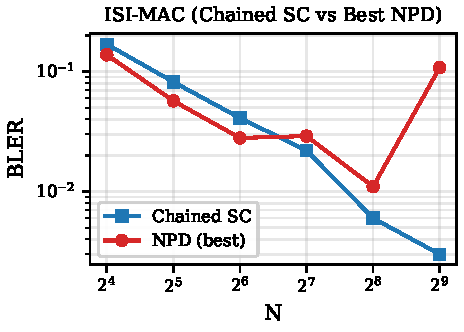
\includegraphics[width=0.75\textwidth]{plot_isi_mac.pdf}
\end{figure}

%% ============================================================
\section{MA-AGN MAC}

$Z_i = (1{-}2X_i) + (1{-}2Y_i) + N_i$, \; $N_i = \alpha \cdot N_{i-1} + W_i$ \; (AR(1) noise).\\
SNR $= 6$\,dB. Continuous state (no analytical trellis).\\
Path: \texttt{make\_path(N, N)} (Class~C corner).\\
Baseline: memoryless GMAC SC (ignores noise correlation).

\subsection*{$\alpha = 0.3$ (weak memory)}

\begin{table}[h]\centering\small
\begin{tabular}{@{}r r r r r@{}}
\toprule
$N$ & $k_u / k_v$ & Memoryless SC & NPD (d=16 h=100) & \textbf{NPD/SC} \\
\midrule
 16 & 4 / 7 & 0.175 & \textbf{0.138} & \textbf{0.79$\times$} \\
 32 & 7 / 15 & 0.057 & 0.053 & 0.93$\times$ \\
 64 & 15 / 29 & 0.025 & 0.036 & 1.42$\times$ \\
128 & 30 / 58 & 0.008 & 0.093 & 11.6$\times$ \\
\bottomrule
\end{tabular}
\end{table}

\begin{figure}[h]\centering
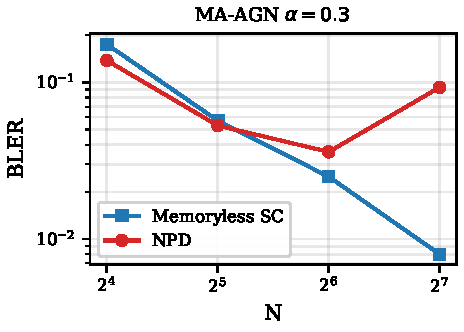
\includegraphics[width=0.75\textwidth]{plot_maagn_03.pdf}
\end{figure}

\subsection*{$\alpha = 0.9$ (strong memory)}

\begin{table}[h]\centering\small
\begin{tabular}{@{}r r r r r@{}}
\toprule
$N$ & $k_u / k_v$ & Memoryless SC & NPD (d=16 h=100) & \textbf{NPD/SC} \\
\midrule
 16 & 4 / 7 & 0.197 & \textbf{0.131} & \textcolor{wingreen}{\textbf{0.66$\times$}} \\
 32 & 7 / 15 & 0.074 & \textbf{0.056} & \textcolor{wingreen}{\textbf{0.76$\times$}} \\
 64 & 15 / 29 & 0.043 & \textbf{0.027} & \textcolor{wingreen}{\textbf{0.62$\times$}} \\
128 & 30 / 58 & 0.028 & 0.061 & 2.18$\times$ \\
\bottomrule
\end{tabular}
\end{table}

\begin{figure}[h]\centering
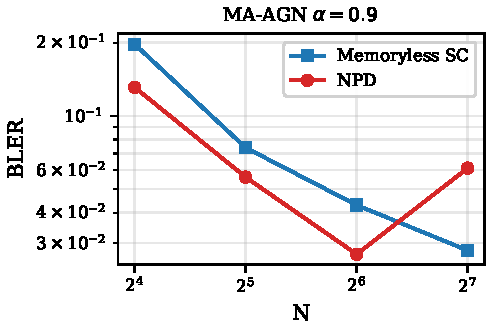
\includegraphics[width=0.75\textwidth]{plot_maagn_09.pdf}
\end{figure}

%% ============================================================
\section*{Summary}

\begin{center}\small
\begin{tabular}{@{}l l l@{}}
\toprule
Channel & NPD vs baseline & $N$ range \\
\midrule
ISI-MAC (d=16 h=100) & 0.68--0.82$\times$ chained trellis SC & $N = 16$--64 \\
ISI-MAC (d=64 h=128) & 1.3--1.8$\times$ chained trellis SC   & $N = 128$--256 \\
MA-AGN $\alpha=0.9$  & 0.62--0.76$\times$ memoryless SC       & $N = 16$--64 \\
MA-AGN $\alpha=0.3$  & 0.79$\times$ memoryless SC              & $N = 16$ only \\
\bottomrule
\end{tabular}
\end{center}

\end{document}
